%===============================================================================
% PREAMBOLO
%===============================================================================

% === Impostazione del documento ===============================================
\documentclass[12pt,a4paper,oneside,english,hidelinks]{book}
\pagenumbering{arabic}
\usepackage{setspace}
\onehalfspace

% === Regolazione dei margini ==================================================
\addtolength{\oddsidemargin}{30pt}
\addtolength{\evensidemargin}{-30pt}
\usepackage{fancyhdr}
\usepackage{multirow}
\usepackage{multicol}
\usepackage[section]{placeins}

% === Impostazione dei font ====================================================
\usepackage[T1]{fontenc}
\usepackage[utf8]{inputenc}
\usepackage[english]{babel}
\usepackage{ae}
\usepackage{relsize}
\usepackage{csquotes}
\usepackage{amsmath}
\usepackage{amsfonts}
\usepackage{mathdots}
\usepackage{mathtools}
\usepackage[colorlinks=true]{hyperref}
\hypersetup{
	bookmarksnumbered=true,
	linkcolor=black,
	citecolor=black,
	%pagecolor=black,
	urlcolor=black,
}
\usepackage{verbatim}
\usepackage{alltt}
\DeclareMathOperator{\sgn}{sgn}
\DeclarePairedDelimiter{\abs}{\lvert}{\rvert}
\DeclarePairedDelimiter{\norma}{\lVert}{\rVert}
\setlength{\parindent}{0pt}

% === Integrazione delle figure ================================================
\usepackage{graphicx}
\graphicspath{{./imgs/}}
\renewcommand{\figurename}{Fig.}
\usepackage{caption}
\usepackage{subfig}


% === Per gli algoritmi ========================================================
\usepackage{algorithmicx}
\usepackage[ruled]{algorithm}
\usepackage{algpseudocode}

% === Per le tabelle ===========================================================
\usepackage{tabularx}
\usepackage{siunitx}
\usepackage{booktabs, array}

% === Per la bibliografia multicolonna =========================================
\usepackage{etoolbox}
\patchcmd{\thebibliography}{\list}{\begin{multicols}{2}\smaller\list}{}{}
\appto{\endthebibliography}{\end{multicols}}
%== Per le figure TikZ e PGF ===================================================
\usepackage{tikz,fp,ifthen,fullpage}
\usepackage{pgfmath}
\usepackage{pgfplots}
\usetikzlibrary{backgrounds}
\usetikzlibrary{decorations.pathmorphing,decorations.markings} 
\usetikzlibrary{backgrounds,fit,calc,through}
\usetikzlibrary{arrows,patterns}
\usetikzlibrary{shapes,decorations,shadows}
\usetikzlibrary{fadings}
\usetikzlibrary{mindmap}
\usetikzlibrary{decorations.text}
\usetikzlibrary{decorations.shapes}
\pgfplotsset{compat=1.13}

%===============================================================================
% TESTO DELLA TESI
%===============================================================================

\begin{document}
	% === Frontespizio ===========================================================
	\pagestyle{empty}
	%%%%%%%%%%%%%%%%%%%%%%%%%%%%%%%%%%%%%%%%%%%%%%%%%%%%%%%%%%%
% Frontespizio
%%%%%%%%%%%%%%%%%%%%%%%%%%%%%%%%%%%%%%%%%%%%%%%%%%%%%%%%%%%
\begin{titlepage}
 \begin{center}
 
\includegraphics[width=3.5cm]{unitn.jpg}\\
 \vspace{1em}
 {\Large \textsc{Università degli studi di Trento}}\\
 \vspace{1em}
 {\Large \textsc{Dipartimento di Ingegneria Industriale}}\\
 \vspace{4em}
 {\normalsize Relazione}\\
 \vspace{1em}
 {\Large \textsc{Mechanical Vibrations}}\\
 \vspace{4em}
 {\LARGE\textbf{
 	System identification of a 3 DOF system
 }}\\
 \end{center}

\vskip 2.0cm
 \begin{center}
 \begin{tabular}{c c c c c c c c}
 Relatore & & & & & & & Candidato \\[0.2cm]
 \large{Prof. Daniele Bortoluzzi} & & & & & & & \large{Francesco Aregntieri}\\[0.4cm]
 Correlatore & & & & & & & ID: 183892\\[0.2cm]
 \large{Dott. Egidio Labbate}& & & & & & &\\
 \end{tabular}
 \end{center}

\vskip 1.5cm
\begin{center}
{\normalsize Anno Accademico 2015/2016}
\end{center}
\end{titlepage}

\clearpage{\pagestyle{empty}\cleardoublepage}

	% === Indice =================================================================
	\tableofcontents

	% === Capitoli Tesi ==========================================================
	\pagestyle{plain}
	\chapter{Introduction}
\label{chap:Introduction}

\section{System and the experimental setup}
\label{sec:intro1}

For this experiment, we are going to identify the parameters of the Rectilinear
Control System (Model 210).
The experimental control system is comprised of the three subsystems shown in
Figure \ref{fig:dynamicalsystem}. The first of these is the electromechanical
plant which consists of the spring/mass mechanism, its actuator and sensors.
The design features a brushless DC servomotor, high resolution encoders,
adjustable masses, and reconfigurable plant type.
%
\begin{figure}[ht]
\centering
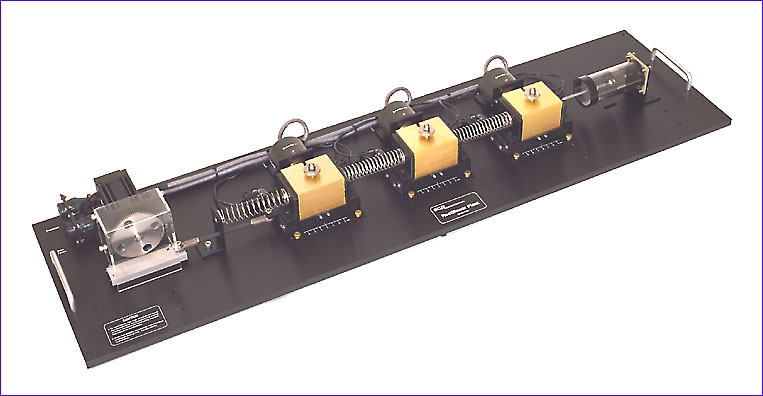
\includegraphics[width=0.8\linewidth]{linlrge}
\caption{Dynamical system}
\label{fig:dynamicalsystem}
\end{figure}
\subsection{Parameters}
The system is configured with three bodies above the mass carriage suspension
is an anti-friction ball bearing type with approximately $\pm 3$
[\si{\centi\meter}] of available travel.
The linear drive is comprised of a gear rack suspended on an anti-friction
carriage and pinion (pitch diameter 7.62 [\si{\centi\meter}]) coupled to the
brushless servo-motor shaft.
Optical encoders measure the mass carriage positions - also via a rack and
pinion with a pinion pitch about 3.18 [\si{\centi\meter}].
The bodies are connected by known stiffness springs, and a spring connects the
third mass to the frame. Instead, the first body is rigidly connected to a
pinion gear with a live-powered motor with a PC interface.
The position of each body is provided by an encoder. The position zeros are at
the equilibrium positions of the springs.
For the springs we use the nominal values provided:
%
\begin{itemize}
	\item $k_1 = k_2 = 800$ [\si{\newton\per\meter}] between $m_1$ and $m_2$, $m_2$
and $m_3$;
	\item $k_3 = 400$ [\si{\newton\per\meter}] between $m_3$ and the ground.
\end{itemize}
%
The shifts $x_1$, $x_2$, $x_3$ are provided in encoder counts, where the
relationship (\ref{eq:encodercounts}) between the measured counts and the
displacement was used.
Where $r_{e}$ is the radius of the encoder and $2\pi r_{e} = 0.0706$
[\si{\meter}]; 16000 is the number of counts per encoder revolution.
%
\begin{equation}
	\Delta x = 2\pi \cdot r_{e} \cdot \frac{\Delta count}{16000}
	\label{eq:encodercounts}
\end{equation}
%
The input data are given by the voltage \si{\volt}.
The following relation between the applied voltage and the applied force holds:
$f = (k_a \cdot k_t \cdot k_{mp}) \cdot v$.\\
Where:\begin{description}
	\item $k_a$ is the Servo Amp gain:
	\begin{equation*}
		k_a \approx 2 \quad [\text{\si{\ampere\per\volt}}]
	\end{equation*}
	\item $k_t$ is the Servo Motor Torque constant:
	\begin{equation*}
		k_t	\approx	0.1 \quad 	[\text{\si{\newton\meter\per\ampere}}]
	\end{equation*}
	\item $k_{mp}$ is the Motor Pinion pitch radius inverse:
	\begin{equation*}
		k_{mp} 	= 26.25 \quad	[\text{\si{\per\meter}}]
	\end{equation*}
\end{description}

\section{The dynamical model}
\label{sec:dynamicalmodel}

\subsection{Assumption}
\label{subsec:assumption}
The system described in the previous chapter is modelled as a linear system and
for this reason some simplifications are made.
It is considered that all the bodies move on the same axis, assuming therefore
that the rack meshed by the pinion plots the force on this axis, so that a
straight motion is assumed.
In the model there are only viscous frictions.
The block containing the engine with the attachment unit and rack is considered
rigidly connected to the mass m, according to the equation:
\begin{equation}
	\label{eq:reducedinertia}
	\begin{cases}
		m_{1} &=  m_{11} + \frac{J_{\text{motor}}}{r^2}\\
		c_{1} &=  c_{11} + \frac{c_{\text{motor}}}{r^2}
	\end{cases}
\end{equation}
In equation \eqref{eq:reducedinertia}: $r$ is the radius of the pinion-rack
coupling, $J_{\text{motor}}$ the inertia of the motor, $c_{\text{motor}}$ the
rotational damping.
While $m_{11}$ and $c_{11}$ are respectively the mass and damping of the first body.
%
\subsection{Equation of motion}
\label{subsec:equationofomotion}
We describe the equations of motion for each body according to the embodiments
reported in \eqref{eq:equationmotion}, the schematic representation is
observable in the figure \ref{fig:modelscheme}
%
\begin{equation}
	\label{eq:equationmotion}
	\begin{array}{l}
		m_1 \ddot{x}_{1} = k_1 (x_2 - x_1) - c_1 \dot{x}_{1} + g_{\text{v}} \cdot v	\\
		m_2 \ddot{x}_{2} = k_1 (x_1 - x_2) + k_2 (x_3 - x_2) - c_2 \dot{x}_{2} \\
		m_3 \ddot{x}_{3} = k_2 (x_2 - x_3) - c_3 \dot{x}_{3} - k_3 x_3	\\
	\end{array}
\end{equation}
%
The equation in matrix form is shown below (\ref{eq:matrixform}):
%
\begin{equation}
	\label{eq:matrixform}
	\begin{bmatrix}
		m_1	&  	0	&	0	\\
 		0	& 	m_2	&	0	\\
 		0	&  	0	&	m_3	\\
	\end{bmatrix}
	\ddot{x}+
	\begin{bmatrix}
		c_1	&	0	&	0	\\
  		0	&	c_2	&  	0	\\
  		0	&	0	& 	c_3	\\
	\end{bmatrix}
	\dot{x}+
	\begin{bmatrix*}[c]
		k_1		&	-k_1			&       0	\\
 		-k_1		& 	k_1 + k_2	&     -k_2	\\
  		0		&	-k_2			& k_2 + k_3	\\
	 \end{bmatrix*}
 	x=\begin{bmatrix}
 	g_{\text{v}}	\\
 	0 	\\
 	0
 	\end{bmatrix} \cdot v
\end{equation}
%
\begin{figure}[hb]
	\centering
    \resizebox{.8\linewidth}{!}{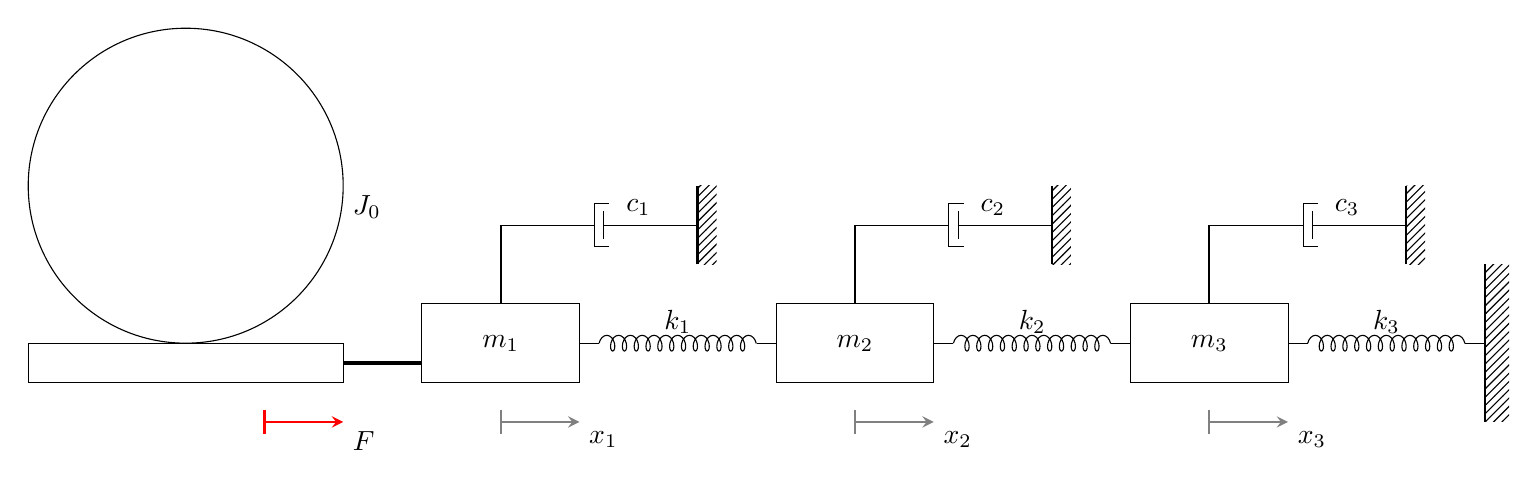
\begin{tikzpicture}
%\draw[help lines] (0,0) grid [step = 5 mm](15,3.5);
%\foreach \x in {0,1,...,15}
%   \draw [help lines] (\x,0) node [below,%
%          font=\footnotesize] {$\x$} -- (\x,0);
%\foreach \y in {0,1,...,3.5}
%   \draw [help lines] (0,\y) node [left,%
%          font=\footnotesize] {$\y$} -- (0,\y);

% Define style for spring
\tikzstyle{springshape}=[decoration={aspect=0.6, segment length=1.5mm, amplitude=1mm, coil}, decorate];
\newcommand{\spring}[3]{%
	% pass 3 arguments:
	% arg1: #1 coordinate x; arg2:  #2 coordiante y; arg3: #3 number of componets
	\coordinate (attachleftside) at ({#1},{#2});
	\coordinate (startspring) at ($(attachleftside) + (0.25,0)$);
	\coordinate	(endspring) at ($(startspring) + (2,0)$);
	\coordinate	(attachrightside) at ($(endspring) + (0.25,0)$);
	\draw (attachleftside) -- (startspring);
	\draw [springshape] (startspring) -- (endspring) node[draw=none,pos=0.5, above] (){$k_{#3}$};
	\draw (endspring) -- (attachrightside);
}

% Define style for dampers
\tikzstyle{dampshape}=[decoration={markings, mark connection node=dmp,
  mark=at position 0.5 with
  {
    \node (dmp) [inner sep=0pt,transform shape,rotate=-90,minimum width=15pt,minimum height=3pt,draw=none] {};
    \draw  ($(dmp.north east)+(2pt,0)$) -- (dmp.south east) -- (dmp.south west) -- ($(dmp.north west)+(2pt,0)$);
    \draw ($(dmp.north)+(0,-5pt)$) -- ($(dmp.north)+(0,5pt)$);
  }
}, decorate]
\newcommand{\dampers}[3]{%
	% pass 3 arguments:
	% arg1: #1 coordinate x; arg2: #2 coordiante y; arg3: #3 number of componets
	\coordinate (attachleftside) at ({#1},{#2});
	\coordinate (startdamp) at ($(attachleftside) + (0.25,0)$);
	\coordinate	(enddamp) at ($(startdamp) + (2,0)$);
	\coordinate	(attachrightside) at ($(enddamp) + (0.25,0)$);
	\draw (attachleftside) -- (startdamp);
	\draw [{dampshape}] (startdamp) -- (enddamp) node[draw=none,pos=0.75, above] (){$c_{#3}$};
	\draw (enddamp) -- (attachrightside);
}

% draw gear
\newcommand{\gear}[3]{%
  \def\modu{#1mm}
  \def\Zb{#2}
  \def\AngleA{#3}

  \pgfmathsetmacro{\Rpr}{\Zb*\modu/2}
  \pgfmathsetmacro{\Rb}{\Rpr*cos(\AngleA)}
  \pgfmathsetmacro{\Rt}{\Rpr+\modu}
  \pgfmathsetmacro{\Rp}{\Rpr-1.25*\modu}
  \pgfmathsetmacro{\AngleT}{pi/180*acos(\Rb/\Rt)}
  \pgfmathsetmacro{\AnglePr}{pi/180*acos(\Rb/\Rpr)}
  \pgfmathsetmacro{\demiAngle}{180/\Zb}
  \pgfmathsetmacro{\Angledecal}{(\demiAngle-2*\AnglePr)/2}

  \foreach \zz in{1,2,...,\Zb}{
    \draw
    ({(\zz))/\Zb*360-\Angledecal}:\Rb)
    -- (\zz/\Zb*360-\Angledecal:\Rp)
    to[bend right=\demiAngle]
    (\zz/\Zb*360+\Angledecal:\Rp)
    --
    plot[domain=-0:\AngleT,smooth,variable=\t]
    ({{180/pi*(-\t+tan(180/pi*\t)) +\zz/\Zb*360+\Angledecal}:\Rb/cos(180/pi*\t)})
    %
    to[bend right=\demiAngle]
    ({{180/pi*(\AngleT+tan(180/pi*-\AngleT)) +(\zz+1)/\Zb*360-\Angledecal}:
      \Rb/cos(180/pi*-\AngleT)})
    %
    plot[domain=-\AngleT:-0,smooth,variable=\t]
    ({{180/pi*(-\t+tan(180/pi*\t)) +(\zz+1)/\Zb*360-\Angledecal}:\Rb/cos(180/pi*\t)});
  }
}

% Define ground
\tikzstyle{ground}=[fill,pattern=north east lines,draw=none,minimum width=2cm,minimum height=0.3cm, rotate=90];
\tikzstyle{groundc}=[fill,pattern=north east lines,draw=none,minimum width=10mm,minimum height=0.2cm, rotate=90];
\begin{scope}[xshift=-3cm]
	\draw  (0,2.5) circle (2);
	\node [draw=none, anchor = north west] at (2,2.5) {$J_{0}$};
	\draw  (-2,0) rectangle (2,0.5);
	\draw[ultra thick] (2,0.25) -- (3,0.25);
	\draw [thick, red](1,-0.35)--(1,-0.65);
	\draw [-stealth, thick, red] (1,-0.5) -- (2,-0.5);
	\node [draw=none, anchor = north west] at (2,-0.5) {$F$};
\end{scope}
% generate plot
\begin{scope}[xshift=0cm]
	\draw (0,0) rectangle (2,1) node[draw=none,pos=0.5] () {$m_{1}$};
	\spring{2}{0.5}{1};
	\dampers{1}{2}{1};
	\draw [thick] (3.5,1.5) -- (3.5,2.5);
	\node [groundc,anchor=north]  at (3.5,2){};
	\draw [thick] (1,1) -- (1,2);
	\draw [thick, gray](1,-0.35)--(1,-0.65);
	\draw [-stealth, thick, gray] (1,-0.5) -- (2,-0.5);
	\node [draw=none, anchor = north west] at (2,-0.5) {$x_1$};
\end{scope}
\begin{scope}[xshift=4.5cm]
	\draw (0,0) rectangle (2,1) node[draw=none,pos=0.5] () {$m_{2}$};
	\spring{2}{0.5}{2};
	\dampers{1}{2}{2};
	\draw [thick] (3.5,1.5) -- (3.5,2.5);
	\node [groundc,anchor=north]  at (3.5,2){};
	\draw [thick] (1,1) -- (1,2);
	\draw [thick, gray](1,-0.35)--(1,-0.65);
	\draw [-stealth, thick, gray] (1,-0.5) -- (2,-0.5);
	\node [draw=none, anchor = north west] at (2,-0.5) {$x_2$};
\end{scope}
\begin{scope}[xshift=9cm]
	\draw (0,0) rectangle (2,1) node[draw=none,pos=0.5] () {$m_{3}$};
	\spring{2}{0.5}{3};
	\dampers{1}{2}{3};
	\draw [thick] (3.5,1.5) -- (3.5,2.5);
	\node [groundc,anchor=north]  at (3.5,2){};
	\draw [thick] (1,1) -- (1,2);
	\draw [thick] (4.5,-0.5) -- (4.5,1.5);
	\node [ground,anchor=north]  at (4.5,0.5){};
	\draw [-stealth, thick, gray] (1,-0.5) -- (2,-0.5);
	\draw [thick, gray](1,-0.35)--(1,-0.65);
	\node [draw=none, anchor = north west] at (2,-0.5) {$x_3$};
\end{scope}
\end{tikzpicture}
}
	\caption{model system}
	\label{fig:modelscheme}
\end{figure}

	\chapter{Parameters identification}
\label{chap:paramidentification}
\section{Steady state analysis}
\label{sec:steadystate}
Using the data of the file \emph{data\_steps.mat}, we analysed the step response
of the system by going to check the relationships between the stiffness of the 
springs. 
And estimating a new coefficient for the voltage-to-force.
The estimate of a new voltage-to-force coefficient is carried out using the 
equation \eqref{eq:matrixform}:
\begin{equation} \label{eq:voltage-force}
	[K] x = \begin{bmatrix}
 			g_{\text{v}}	\\
 			0 	\\
 			0
 		\end{bmatrix} \cdot v
\end{equation}
and therefore from \eqref{eq:voltage-force} it is possible to derive:
\begin{equation} \label{eq:voltageforce}
	g_{\text{v}} = [K]^{-1} \cdot b
\end{equation}
Using the steady state value of the three output and the equation 
\eqref{eq:voltageforce} it is possible to evaluate the ratio of the stiffness 
of the springs with respect to  the nominal value of the third spring indicated 
with $k_3$, so it is possible to rewrite:
\begin{equation}
	\label{eq:gvestimate}
	k_3 \begin{bmatrix}
		x_1\\
		x_2\\
		x_3\\
	\end{bmatrix} = v \cdot
	\begin{bmatrix}
		g_{\text{v}} + g_{\text{v}} \cdot \frac{k_3}{k_1} + g_{\text{v}} \cdot 
		\frac{k_{3}}{k_{2}}\\
    		g_{\text{v}} + g_{\text{v}} \cdot \frac{k_{3}}{k_{2}}\\
    		g_{\text{v}}
    \end{bmatrix}
\end{equation}
\begin{figure}[htb]
	\centering
	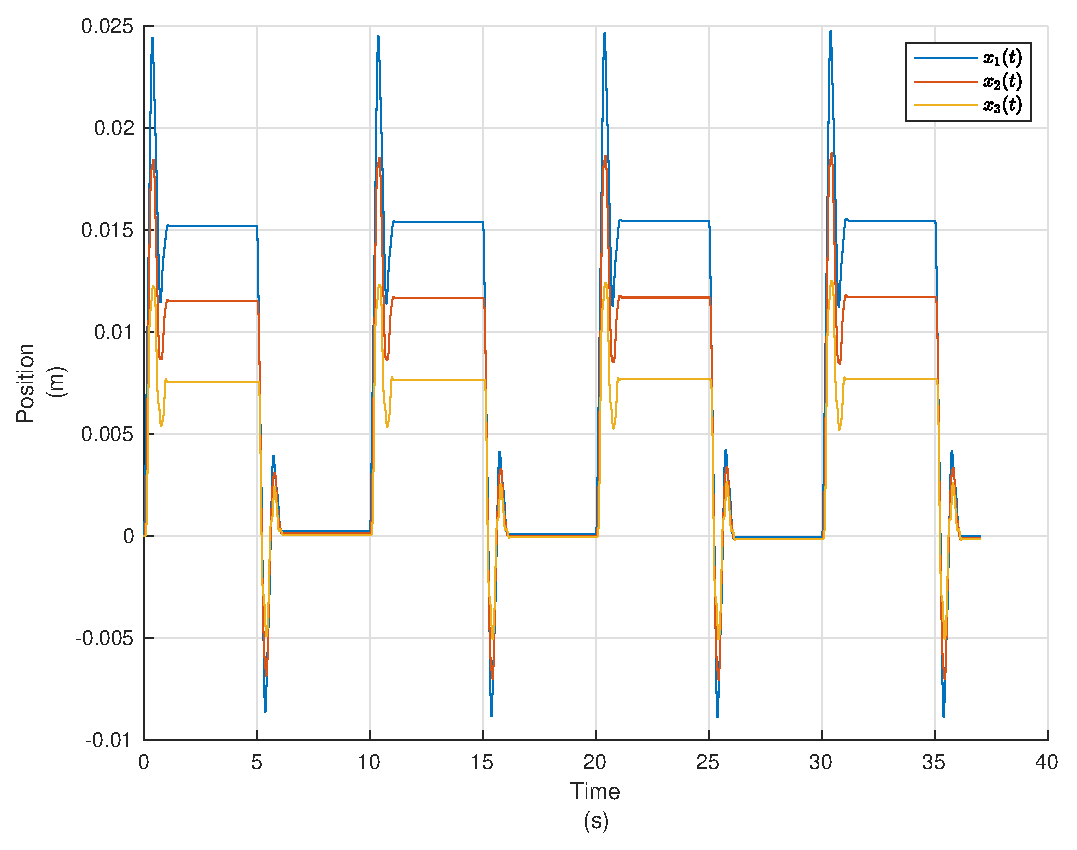
\includegraphics[width=\textwidth]{steadystate}
	\caption{Steady state value pick}
	\label{fig:steadystate}
\end{figure}
From the above equation \eqref{eq:gvestimate} we obtain the results: nominal 
and estimated ratios between the stiffness of the springs as well as the 
coefficient voltage-to-force.
The value of steady state response \(x_{i}\) are picked from the data directly 
in a point far from the transient, as shown in Figure \ref{fig:steadystate}. 
To reduce the zero-mean noise an average with the previous \(400\) samples, i.e.
\(2\) [\si{\second}].
The table \ref{tab:error} shows values and it is possible to appreciate in the 
last column the error made on the estimate of these values, according to the 
formulation:
\begin{equation}
	\label{eq:ratioerror}
	\text{\textbf{err}} = 100\cdot\frac{\text{computed}}{\text{nominal}}
\end{equation}
%
%
\begin{table}[ht]
\centering
	\begin{tabular}{lrrr}
	\toprule
						& nominal & computed & error [\%] \\
 	\midrule
 		ratio $k_{3}/k_{1}$	& 0.50000 & 0.48935 &	2.17651 \\
		ratio $k_{3}/k_{2}$	& 0.50000 & 0.52086 & 	4.00560 \\
		gain ratio $g_{\text{v}}$ & 5.25000 & 6.04866 &  15.21248	\\
	\bottomrule
	\end{tabular}
	\caption{Stiffnesses ratios and voltage-to-force coefficients}
	\label{tab:error}
\end{table}
%
\section{System identification}
\label{sec:sysidentification}
It is necessary to estimate the parameters of three \textsc{dof} system at simple 
identification, so that the impulse response is used to suppose that a model is 
based on a set of parameters, identifying the inputs as the initial force and 
conditions and the output of the system.
thus comparing the system response measured with that predicted by the model.
Defined a model for the system: depends on a set of parameters $\theta$. 
Identify the input (strength and i.c.) and output $(x(t))$ of the system. 
By giving the same input to the model and comparing the measured response $x(t)$ 
to that expected by the model $(x(t,\theta))$.
%
\begin{figure}[htb]
	\centering
	\resizebox{.50\linewidth}{!}{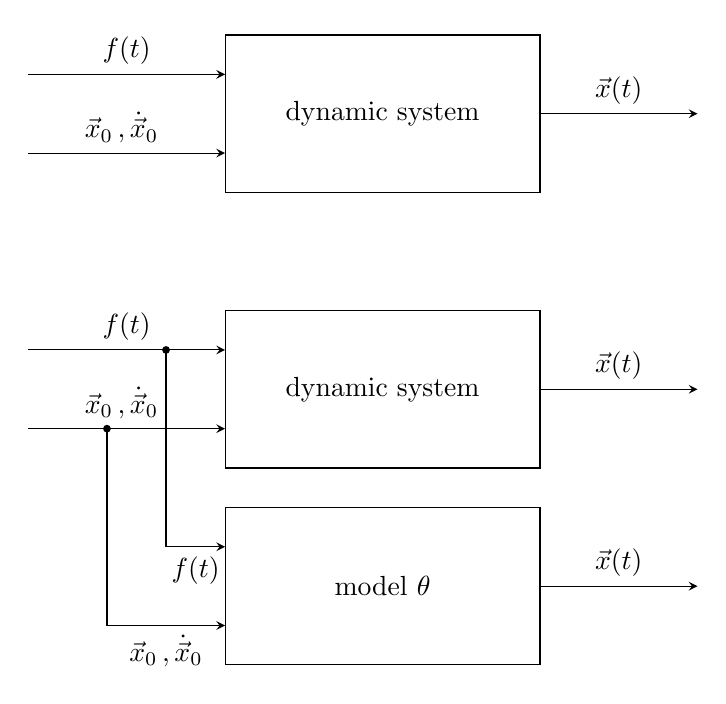
\begin{tikzpicture}
% help guide lines
%\draw[help lines] (0,0) grid [step = 5 mm](10,10);
%\foreach \x in {0,1,...,10}
%   \draw [help lines] (\x,0) node [below,%
%          font=\footnotesize] {$\x$} -- (\x,0);
%\foreach \y in {0,1,...,10}
%   \draw [help lines] (0,\y) node [left,%
%          font=\footnotesize] {$\y$} -- (0,\y);
%
% define model box
\newcommand{\modelbox}[2]{
	% input arrow  
	\coordinate (startarrow) at ({#1},{#2});
	\coordinate	(endarrow) at ($(startarrow)+(2.5,0)$);
	\draw [-stealth]($(startarrow) + (0,1 * 1)$) -- ($(endarrow)+(0,1* 1)$) node[above, midway] {$f(t)$};
	\draw [-stealth]($(startarrow) + (0,1 * 0)$) -- ($(endarrow)+(0,1* 0)$) node[above, midway, xshift=-0.65mm] {$\vec{x}_{0} \,, \dot{\vec{x}}_{0}$};
	% box
	% left low corner
	\coordinate (llcorner) at (2.5,-0.5);
	% right up corner
	\coordinate (rupcorner) at(6.5,1.5);
	\draw (llcorner) rectangle (rupcorner) node [midway]{dynamic system};
	% output arrow
	\coordinate (outputstartarrow) at (6.5,0.5);
	\coordinate	(outputendarrow) at (8.5,0.5);
	\draw [-stealth](outputstartarrow) -- (outputendarrow) node[above, midway] {$\vec{x}(t)$};
};
% 1 - plot the system model
\begin{scope}[yshift = 60mm]
   \modelbox{0}{0};  
\end{scope}
% 2 - plot second model and connection
\begin{scope}[yshift = 25mm]
   \modelbox{0}{0};
   \fill (1.75,1) circle (1.4pt);
   \fill (1,0) circle (1.4pt);
\end{scope}
% connect system model
   \draw (1.75,1) -- (1.75,3.5);
   \draw (1,2.5) -- (1,0);
% box model
\begin{scope}[xshift = 0mm]
   % input arrow  
	\coordinate (startarrow) at (1.75,1);
	\coordinate	(endarrow) at (2.5,1);
	\draw [-stealth](startarrow) -- (endarrow) node[below, midway] {$f(t)$};
	\draw [-stealth](1,0) -- (2.5,0) node[below, midway] {$\vec{x}_{0} \,, \dot{\vec{x}}_{0}$};
	% box
	% left low corner
	\coordinate (llcorner) at (2.5,-0.5);
	% right up corner
	\coordinate (rupcorner) at(6.5,1.5);
	\draw (llcorner) rectangle (rupcorner) node [midway]{model $\theta$};
	% output arrow
	\coordinate (outputstartarrow) at (6.5,0.5);
	\coordinate	(outputendarrow) at (8.5,0.5);
	\draw [-stealth](outputstartarrow) -- (outputendarrow) node[above, midway] {$\vec{x}(t)$};
\end{scope}
\end{tikzpicture}}
	\label{fig:systemmodel}
	\caption{System identification: real system and model}
\end{figure}
%
\\We define the residue as the difference between the two signals as in the 
equation \eqref{eq:residual}.
\begin{equation}
\label{eq:residual}
	\varepsilon(t,\theta) = x(t) - x(t,\theta)
\end{equation} 
The best choice for the set of parameter $\theta$ is the one that minimizes the 
residue integer (\ref{eq:residualinteger}) of the residue. 
\begin{equation}
\label{eq:residualinteger}
	\theta_{optim} = \text{argmin} \biggl( \int \varepsilon(t,\theta)^2 \, dt \biggr)
\end{equation} 
In this case, as the discrete signals with $N$ samples, the optimal value $N$ 
calculated as (\ref{eq:residualdiscrete}), this correspond to solving a least 
square problem.
\begin{equation}
\label{eq:residualdiscrete} 
\theta_{optim} = \text{argmin} \Biggl( \sum_{n=1}^{N} \varepsilon(t,\theta)^2 \Biggr)
\end{equation}

A linear model is adopted as described above, refer \ref{subsec:assumption}, 
assuming the stiffness matrix $[K]$ given.
Then quantifying the $[M]$ and $[C]$ parameters are used to minimize the problem.
Using the \emph{fmincon} algorithm, the problem is resolved. In addition, the 
selected algorithm is required to specify the lower and upper search limits; 
as well as the first guess conditons from which the result is strictly dependent.

\subsection{Free damping case}
\label{subsec:freedamping}
Using the data of the file \emph{data\_impulse.mat} identify the seven parameters
previously identified in the model and described by the equation \eqref{eq:matrixform}. 
In this case, since the response to impulse force, two to approximation of the 
force estimation, will be analysed, the voltage-to-force coefficient will be 
studied again.
The results of this optimization are shown in table \ref{tab:freedamping}.
\begin{table}[ht]
	\centering
	\begin{tabular}{SSSSSSS}
	\toprule
		\multicolumn{1}{c}%
			{$m_1$} & {$m_2$} & {$m_3$} & {$c_1$} &	 {$c_2$} & {$c_3$} & {$g_v$} \\
		\multicolumn{3}{c}{[\si{\kilo\gram}]}	&%
		\multicolumn{3}{c}{[\si{\newton\second\per\meter}]}	&%
		\multicolumn{1}{c}{[\si{\volt}]}\\
	\midrule
          1.5712  & 1.5020  & 1.2018  &  2.7956 &  1.9978 & 2.1950  &  1.2096	\\
    \bottomrule
	\end{tabular}
	\caption{Optimizations results in free damping case}
	\label{tab:freedamping}
\end{table}
\begin{figure}[!htb]
	\centering
	\subfloat[][\emph{mass vs displacement 1.}]
		{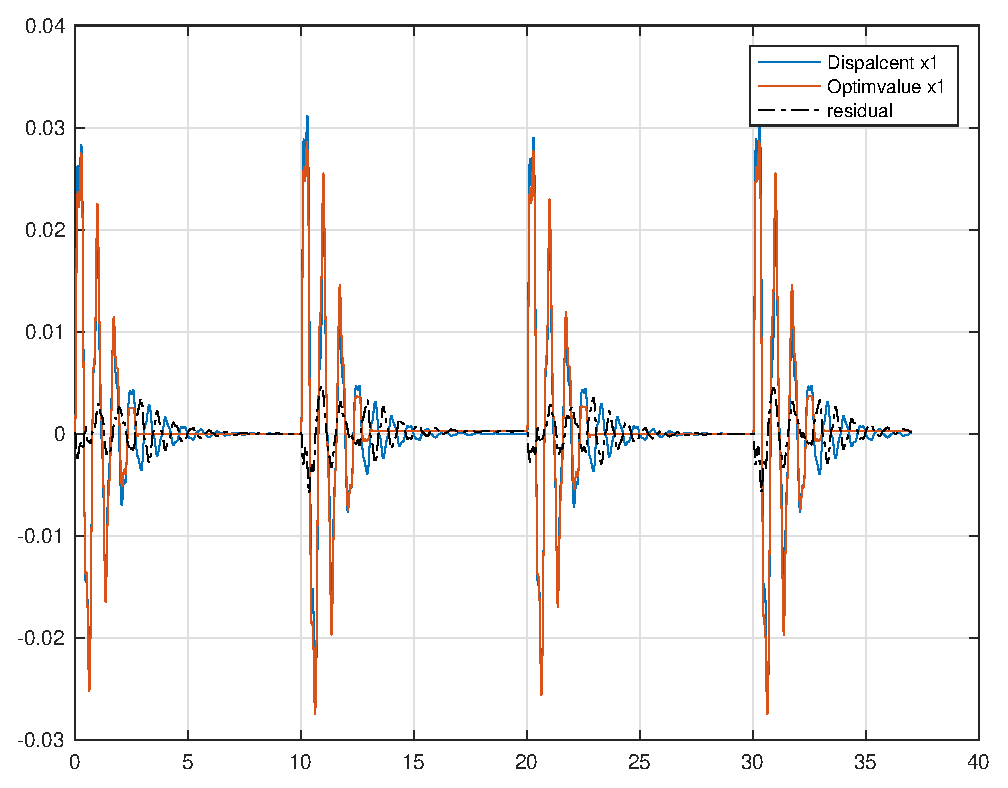
\includegraphics[width=0.75\textwidth]{residualfull1}}	\\
\end{figure}
\begin{figure}[!ht]
	\ContinuedFloat
	\centering
	\subfloat[][\emph{mass vs displacement 2.}]
		{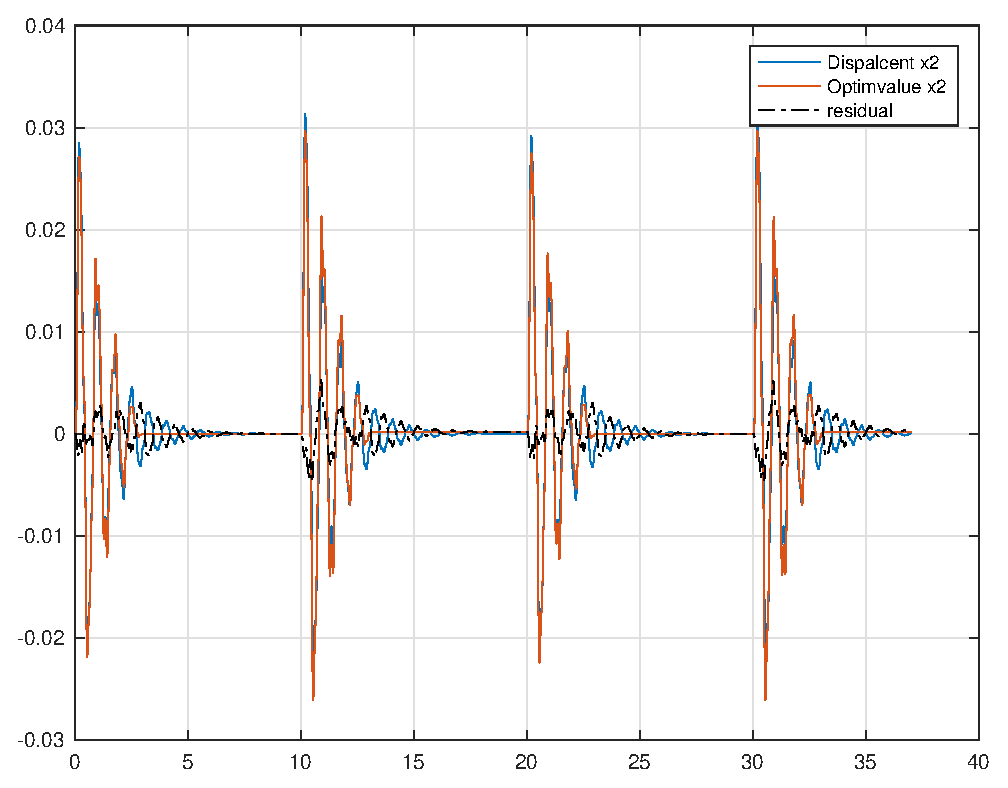
\includegraphics[width=0.75\textwidth]{residualfull2}}	\\
	\subfloat[][\emph{mass vs displacement 3.}]
		{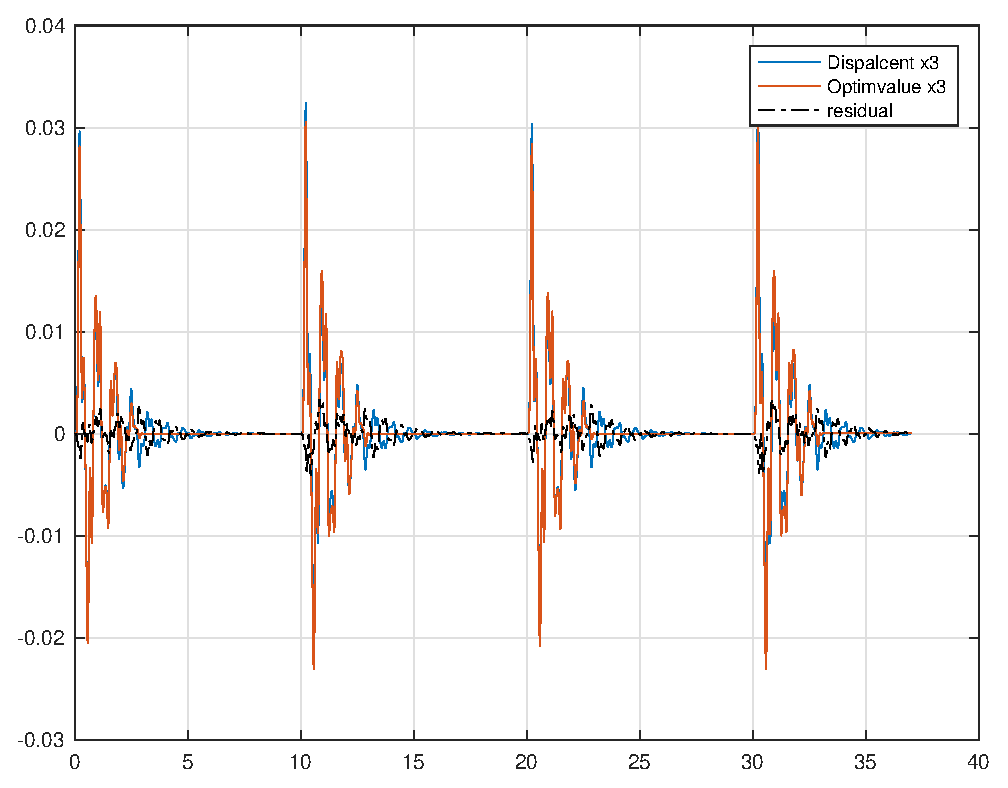
\includegraphics[width=0.75\textwidth]{residualfull3}}
	\caption{Comparison between the response of the model and the response of the 
	system free damping case}
	\label{fig:freedampingcase}
\end{figure}

\subsection{Proportional damping case}
\label{subsec:proportionaldamping}
In this case, the procedure used to solve the problem raised in the case of 
free damping to obtain the parameters is used; changing some conditions.
We define damping through the equation (\ref{eq:proportionaldamping}) where it 
is possible to observe that this depends on the linear combination of the mass 
matrix multiply by constant and the stiffness matrix multiply by the another 
constant.
Then the search limits and first guess will be changed to search the mass 
values and the unknown constants.
The interesting property of this representation is the ability to perform modal 
decomposition on the system.
\begin{equation}
\label{eq:proportionaldamping}
	[C] = \alpha \cdot [M] + \beta \cdot [K]
\end{equation}
The optimization results are available in the table \ref{tab:proportionaldamping}.
%
\begin{table}[htb]
	\centering
	\begin{tabular}{SSSSSS}
	\toprule
	\multicolumn{1}{c}%
			{$m_1$} & {$m_2$} & {$m_3$} & {$g_v$} &	 {$\alpha$} & {$\beta$} \\
	\multicolumn{3}{c}{[\si{\kilo\gram}]}	& %
	\multicolumn{1}{c}{[\si{\volt}]} & %
	\multicolumn{2}{c}{[\si{\newton\second\per\meter}]} \\
	\midrule
       			1.5761   &  1.4970  & 1.1996  &  1.2094 &  1.6209   &  0.0001	\\
    \bottomrule
	\end{tabular}
	\caption{Optimizations results in proportional damping case}
	\label{tab:proportionaldamping}
\end{table}
\begin{figure}[htb]
\centering
	\subfloat[][\emph{mass vs displacement 1.}]
		{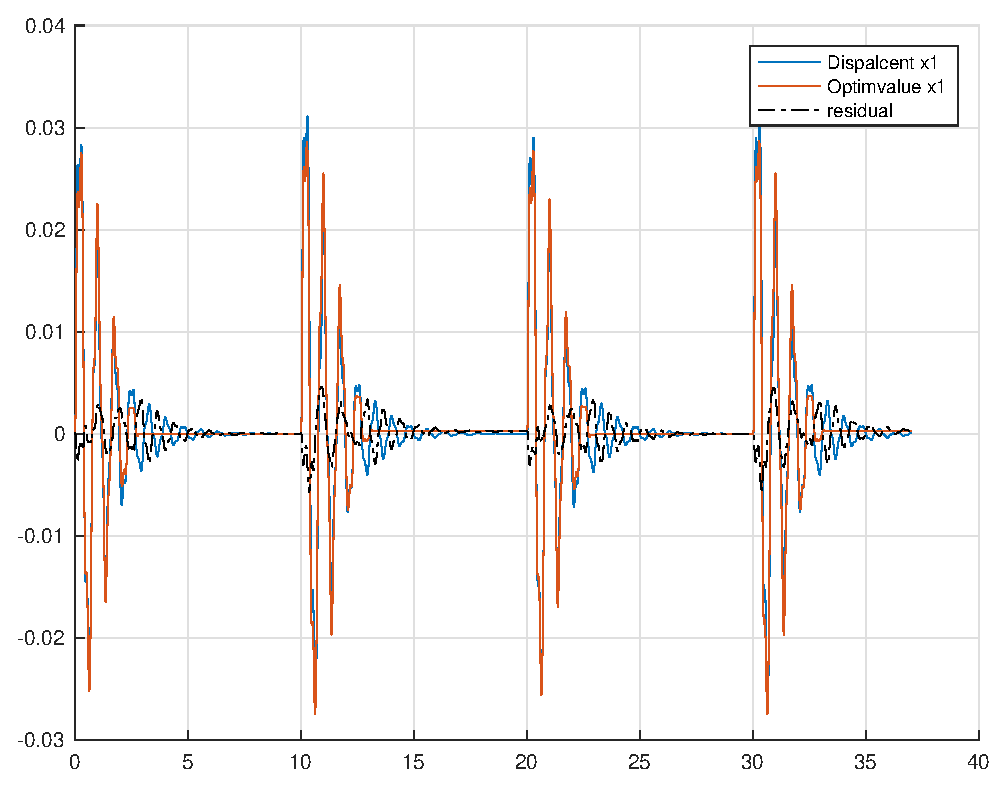
\includegraphics[width=0.75\textwidth]{residualpropdamp1}}	\\
\end{figure}
\begin{figure}[htb]
	\ContinuedFloat
	\centering	
	\subfloat[][\emph{mass vs displacement 2.}]
		{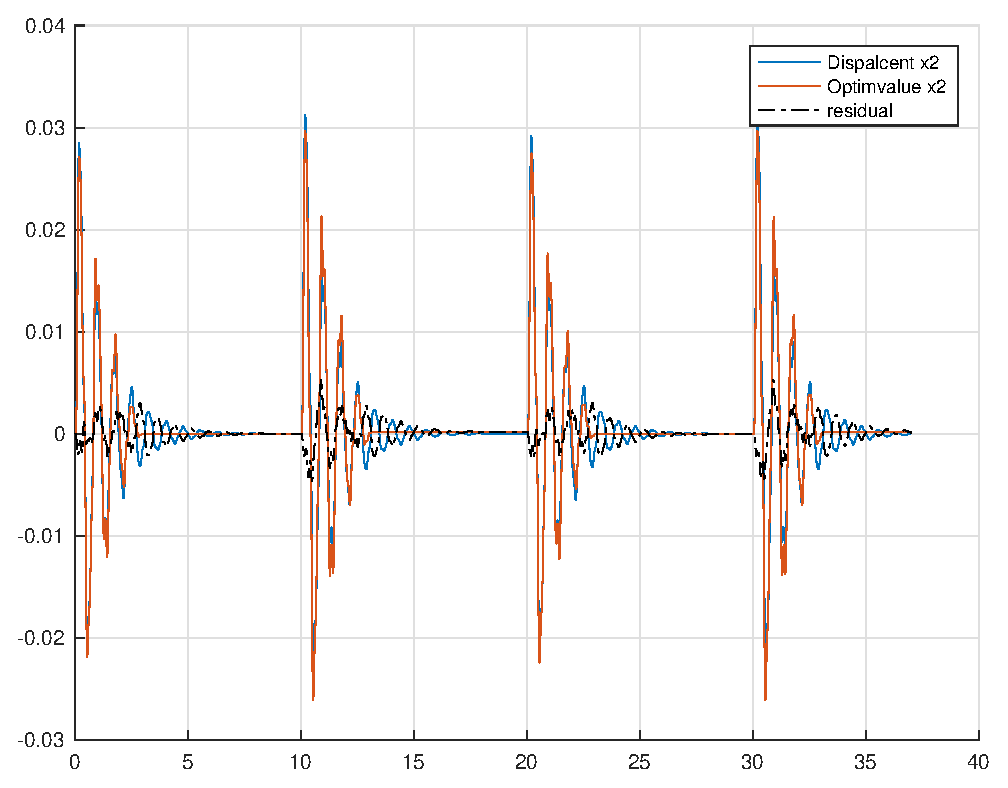
\includegraphics[width=0.75\textwidth]{residualpropdamp2}}	\\
	\subfloat[][\emph{mass vs displacement 3.}]
		{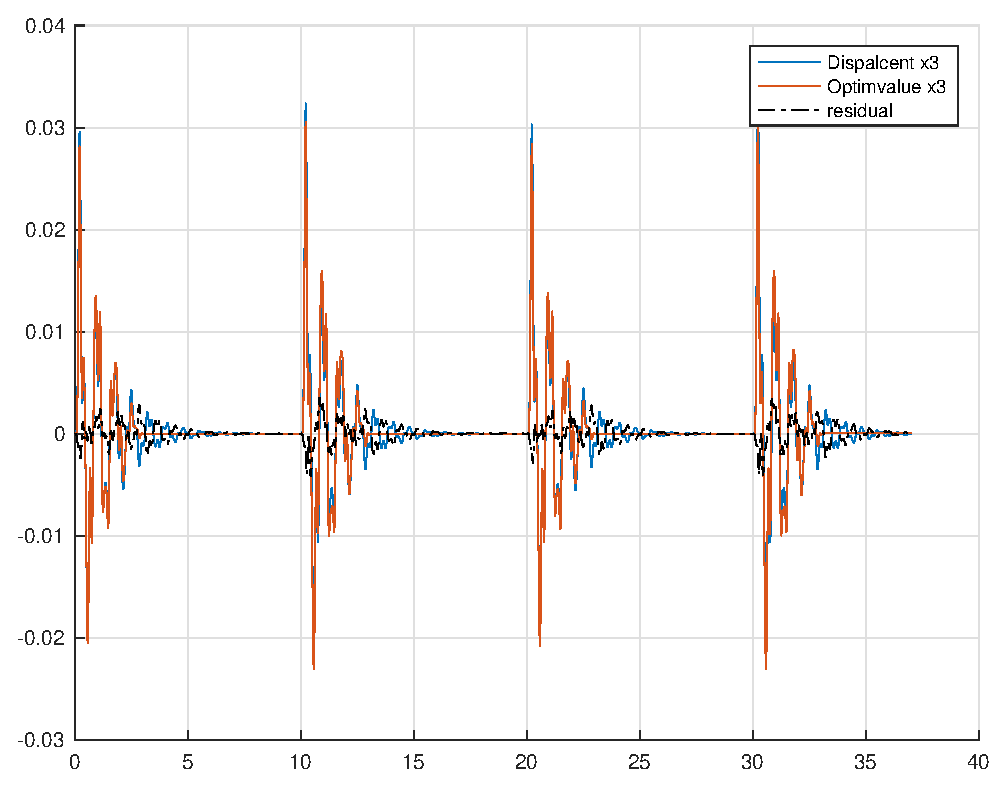
\includegraphics[width=0.75\textwidth]{residualpropdamp3}}	
	\caption{Comparison between the response of the model and the response of the system proportional damping case}
	\label{fig:proportionaldamping}
\end{figure}

%TODO describe the matrix C 
%The matrix [C] is:
\begin{equation}
\label{}
	[C] =
	\begin{bmatrix*}[r]
		 2.64026		&	-0.08550		 & 	 0.00000 	\\
		-0.08550 	&	 2.59748		 &	-0.08550		\\
		 0.00000 	&	-0.08550		 &	 2.07270		\\
	\end{bmatrix*}
\end{equation}
%\pagebreak
%
\subsection{Comparison}
\label{subsec:comparison}
After fitting data with a model, you should evaluate the goodness of fit. 
The goodness of fit is calculated using the normalized root mean square error 
as the cost function.
In table \ref{tab:goodoffit} are available the percentages the measured output.
This method to assess goodness of fit for both linear and non linear parametric 
fits.
As is common in statistical literature, the term goodness of fit is used here 
in sense: ``good fit" might be a model where the data could reasonably have 
come from, given the assumptions of least-squares fitting.
\begin{table}[ht]
\centering
\begin{tabular}{lccc}
	\toprule
		 & $x_1$ [\%] & $x_2$ [\%] & $x_3$ [\%]\\
	\midrule
	% free damping result
	free damping case & 81.36 & 81.17 & 81.71 \\
	% proportianl damping result
	proportinal damping case & 81.36 & 81.17 & 81.56 \\
	\bottomrule
\end{tabular}
\caption{Result \emph{goodness of fit} measured output}
\label{tab:goodoffit}
\end{table}
%
\subsection{Multiple single DOF system case}

	\input{modal}
	\chapter{Transfer Function}\label{chap:tf}
The transfer function was calculated from the system equation
\eqref{eq:equationmotion} analysed in the section
\ref{subsec:equationofomotion}, where the input is \(g_{\text{v}}\).
To calculate the transfer function between the force and the positions, the 
voltage-to-foce coefficient gain has to be removed.
\begin{equation}\label{eq:gs}
	G(s) = \big([M]s^2+[C]s+[K]\big)^{-1}
\end{equation}
Given \(F(s)\) we obtain the Laplace transform of the force signal.
The transfer function is a column vector with three entries, one for each output,
they share the denominator as in eq.\eqref{eq:gs}.
\begin{equation}\label{eq:tf}
	\frac{X(s)}{F(s)} = \frac{1}{g_{\text{v}}}\,\frac{X(s)}{V(s)}
\end{equation}
%
\begin{figure}[htb]
	\centering
	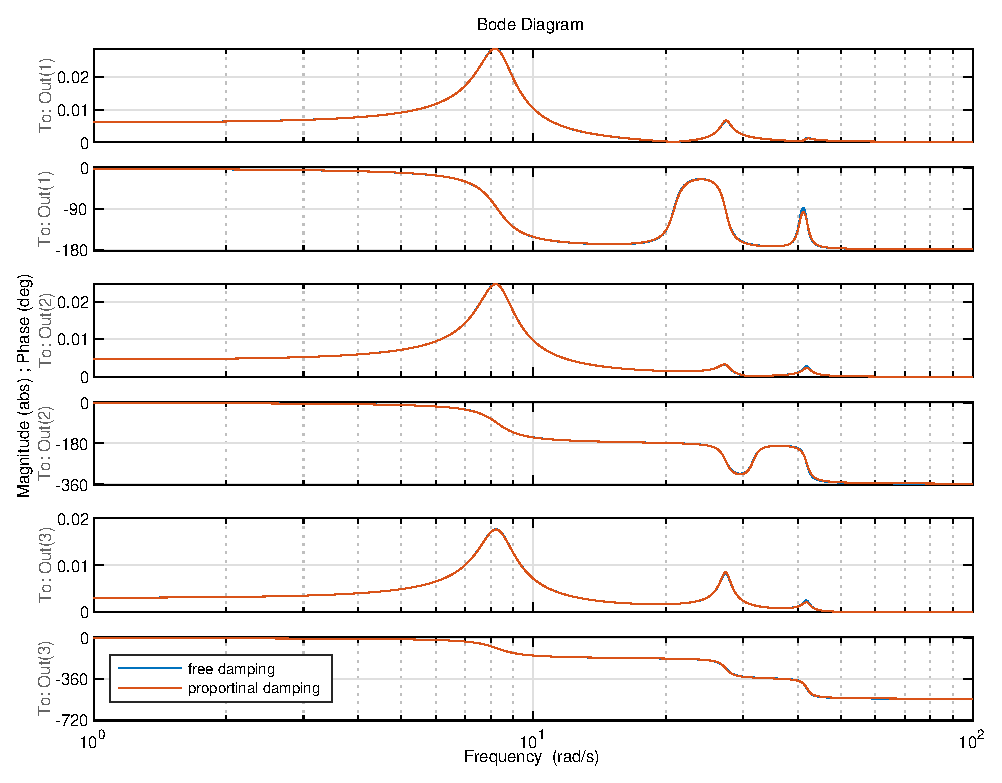
\includegraphics[width=\linewidth]{bodediagram1}
	\caption{Bode diagram of the transfer functions as in \eqref{eq:tf}}
	\label{fig:bodeplot1}
\end{figure}
The bode diagram are shown in Figure \ref{fig:bodeplot1}.
	\chapter{Sinesweep analysis}\label{chap:sinesweep}
The inputs provided are two sine sweep equal signal with different sample
frequencies \(5\) [\si{\milli\second}] and \(10\) [\si{\milli\second}] 
respectively.
To visualize the spectra of the signals, by \emph{fft} is performed on both the
signal.
\begin{figure}[htb]
	\centering
	\subfloat[][\emph{slow}]
		{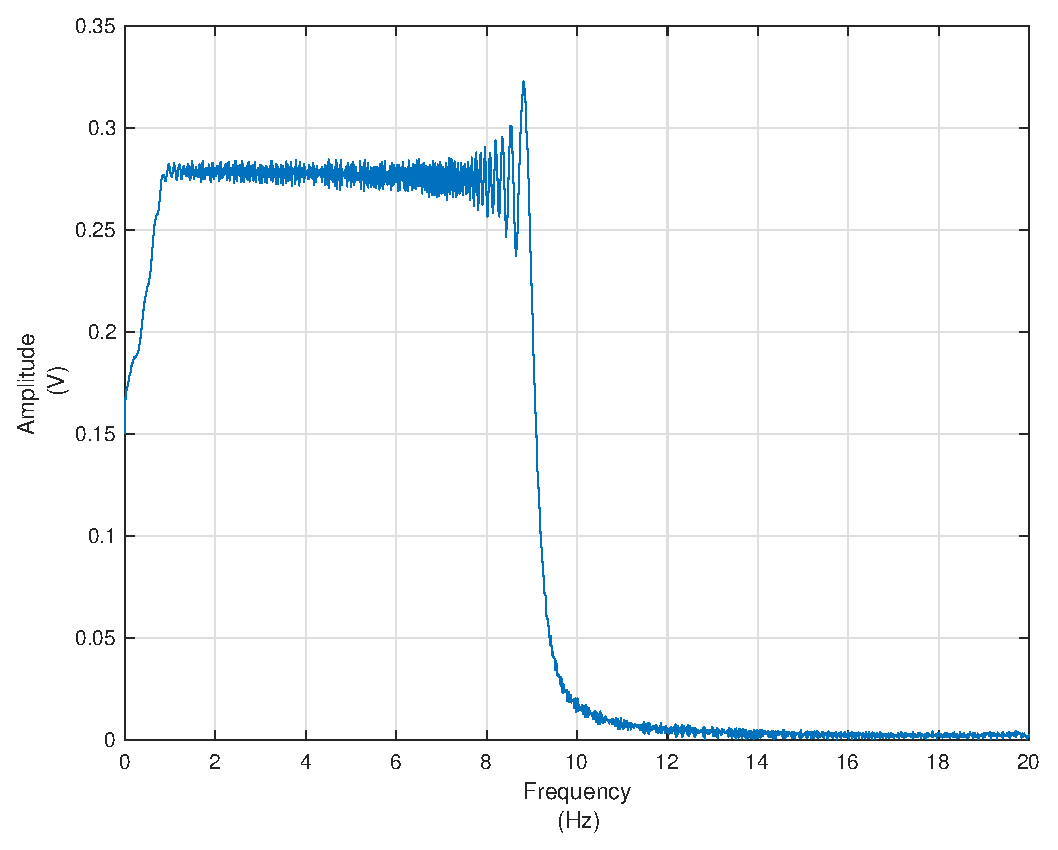
\includegraphics[width=0.45\textwidth]{Fouriertrasformslow}}	\,
	\subfloat[][\emph{fast}]
		{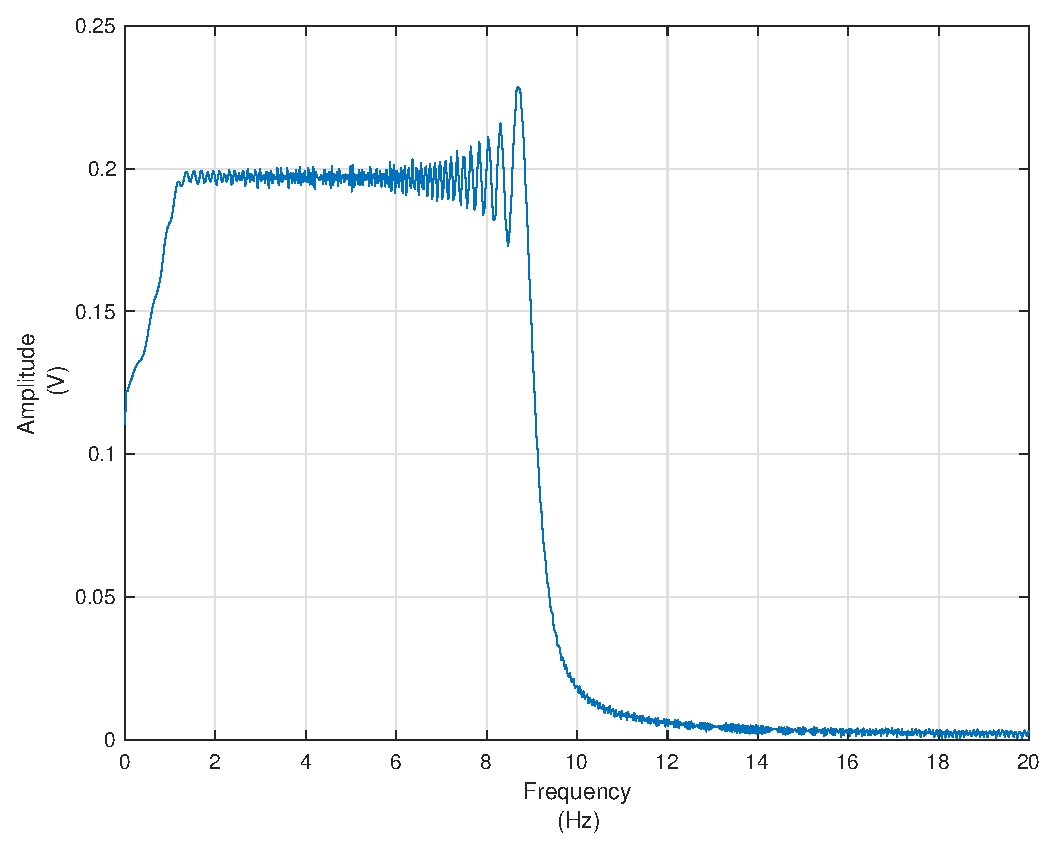
\includegraphics[width=0.45\textwidth]{Fouriertrasformfast}}
	\caption{Sine sweep spectrum}
	\label{fig:spectral}
\end{figure}
The spectrum is plotted with the real frequencies in figure \ref{fig:spectral}.\\
Although the two signals sweep the same frequency range and the difference is
only in the sampling time. These include the resonance peaks of the transfer
function.
On the other hand, the spectrum of the sinusoidal scan excites each frequency
for a limited period of time so it is possible to notice that the third mode is
not clearly visible.
\begin{figure}[htb]
	\centering
	\subfloat[][Respect mass 1]
		{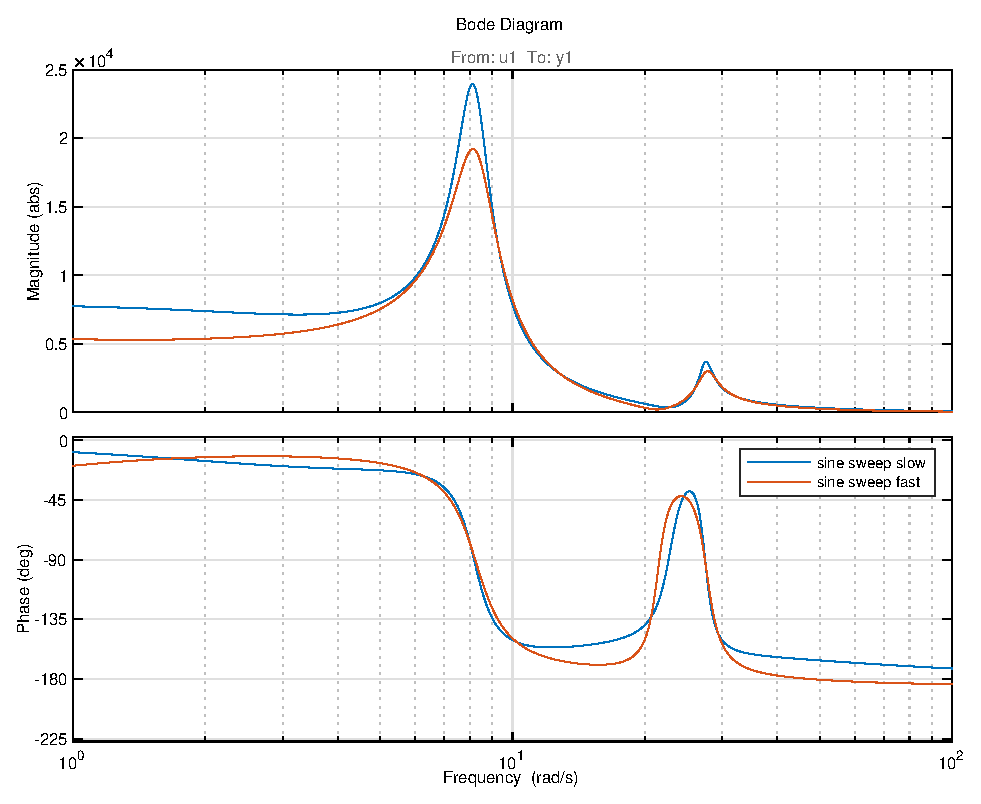
\includegraphics[width=0.5\textwidth]{sinecomparebodediagram1}}	\\
	\subfloat[][Respect mass 2]
		{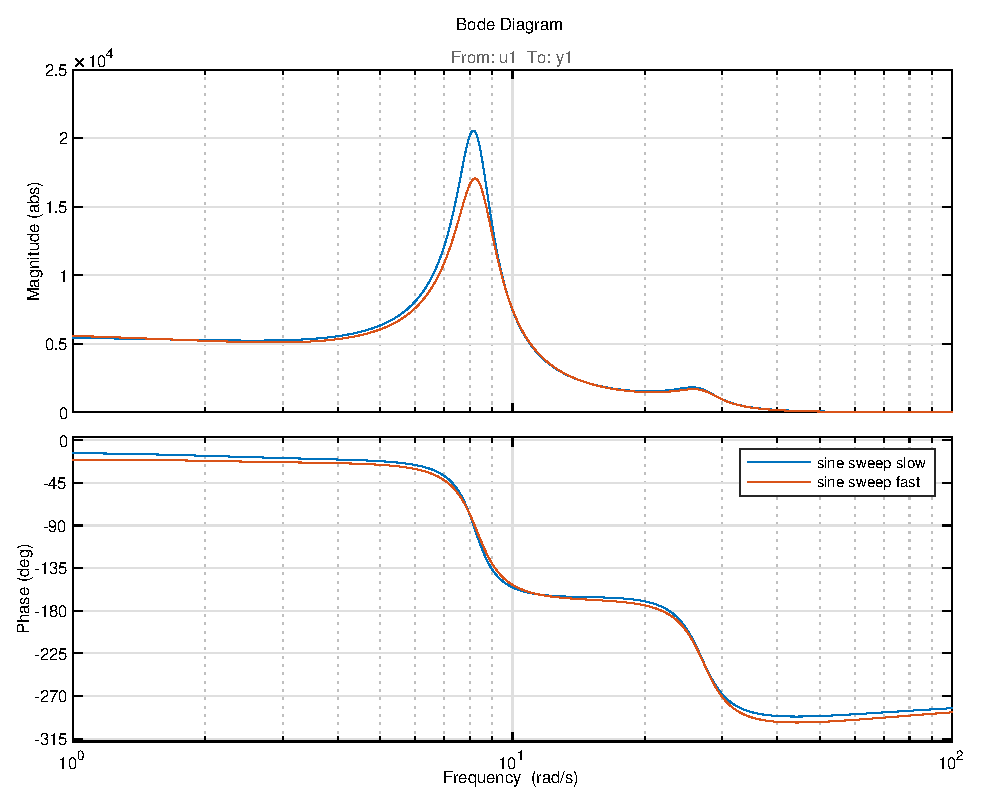
\includegraphics[width=0.5\textwidth]{sinecomparebodediagram2}}	\\
	\subfloat[][Respect mass 3]
		{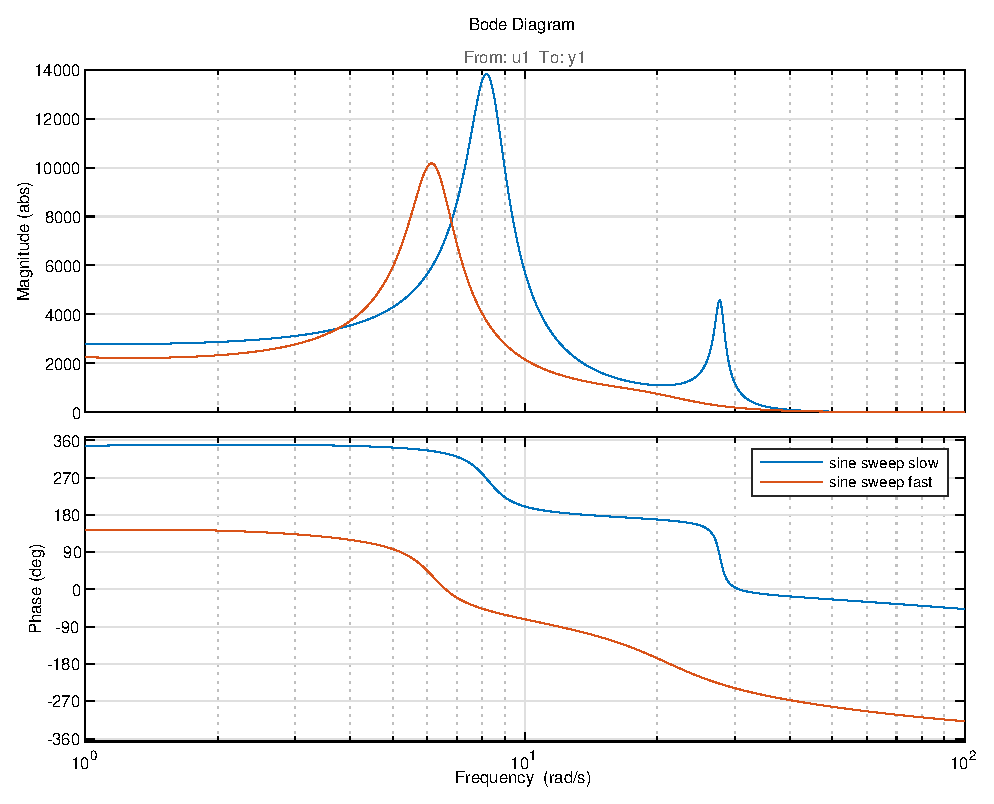
\includegraphics[width=0.5\textwidth]{sinecomparebodediagram3}}	\\
	\caption{Comparison sine sweep outputs of the system}
	\label{fig:bodesinesweep}
\end{figure}


	% === Bibliografia ===========================================================
	\newpage
	\nocite{*}
	\bibliographystyle{IEEEtran}
	\bibliography{bibliografia-tesi.bib}

\end{document}
